\documentclass[11pt,a4paper]{article}

% Packages
\usepackage[utf8]{inputenc}
\usepackage[spanish, es-tabla]{babel}
\usepackage{caption}
\usepackage{listings}
\usepackage{adjustbox}
\usepackage{enumitem}
\usepackage{boldline}
\usepackage{amssymb, amsmath}
\usepackage[margin=1in]{geometry}
\usepackage{xcolor}
%\usepackage{soul}
\usepackage{enumerate}
\usepackage{hyperref}
\usepackage{graphics, graphicx, float}

% Meta
\title{\textbf{\huge Metaheurísticas: Práctica 1 }
	\\\medskip \Large Técnicas de Búsqueda Local y Algoritmos Greedy\\ para el Problema de la Máxima Diversidad \\\medskip}
\author{Pilar Navarro Ramírez - 76592479H \\ pilarnavarro@correo.ugr.es \\ Grupo 2: Viernes de 17:30 a 19:30}
\date{ \today }

% Custom
\providecommand{\abs}[1]{\lvert#1\rvert}
\setlength\parindent{0pt}
\definecolor{Light}{gray}{.90}
\newcommand\ddfrac[2]{\frac{\displaystyle #1}{\displaystyle #2}}
\setlength{\parindent}{1.5em} %sangria
\setlength{\parskip}{3mm}

% Displaying code with lstlisting
\lstset { %
	language=C++,
	backgroundcolor=\color{black!5}, % set backgroundcolor
	basicstyle=\small,% basic font setting
}

\usepackage[ruled]{algorithm2e}


\begin{document}	
	
	\maketitle 
	\newpage
	\tableofcontents
	\newpage
	
	
	\section{Descripción del problema}
	
	
	El \textbf{Problema de la Máxima Diversidad (Maximum Diversity Problem, MDP)}, es un problema NP-completo de optimización combinatoria. 
	Consiste en seleccionar un subconjunto de $m$ elementos de un conjunto inicial de $n$ elementos (con $n>m$) de forma que se maximice la diversidad entre los elementos escogidos.
	
	Además de esto, se dispone de una matriz $D=(d_{ij})$ de dimensión $n\times n$ que contiene las distancias entre todos los $ n $ elementos. Así, en la posición $(i,j)$ de la matriz, se encuentra la distandia entre el elemento i-ésimo y el j-ésimo ($\forall i,j=1,...,n$), siendo $d_{ii}=0\hspace{1mm}\forall i=1,...,n$. Por lo tanto, se trata de una matriz simétrica cuya diagonal está formada por ceros. 
	
	Existen varias formas de calcular la diversidad, pero la que nosotros usaremos consiste en calcular la suma de las distancias entre cada par de elementos de los $m$ seleccionados. 
	
	 El problema MDP se puede formular matemáticamente como sigue:
	
	$$ \text{Maximizar } z_{MS}(x) = \sum_{i=1}^{n-1} \sum_{j=i+1}^{n} d_{ij} x_i x_j $$
	$$ \text{Sujeto a } \sum_{i=1}^{n} x_i = m $$
	$$ x_i \in \{0,1\}, \forall i \in \{1,\dotsc,n\} $$
	
	donde $x$ es una solución al problema, esto es, es un vector binario de longitud $n$ que indica los $m$ elementos seleccionados, donde la posición i-ésima es 1 si se ha seleccionado el elemento i-ésimo.
	
	\newpage

%	\subsection{Casos considerados}
%	
%	Se utilizarán 30 casos seleccionados de varios de los conjuntos de instancias disponibles en la \emph{MDPLIB} (\url{http://www.optsicom.es/mdp/}), 10 pertenecientes al grupo \textbf{GKD} con distancias Euclideas, $n=500$ y $m=50$ ($GKD-c\_i\_n500\_m50$ para $i\in\{1,\dotsc,10\}$), 10 del grupo \textbf{SOM} con distancias enteras entre 0 y 999, $n\in\{300,400,500\}$ y $m=\in\{40,\dotsc,200\}$ ($SOM-b\_11\_n300\_m90$ a $SOM-b\_20\_n500\_m200$) y 10 del grupo \textbf{MDG} con distancias enteras entre 0 y 10, $n=2000$ y $m=200$ ($MDG-a\_i\_n2000\_m200$ para $i\in\{21,\dotsc,30\}$. \\
%	
%	Puesto que la numeración utilizada es unívoca se hará referencia a estas entradas simplemente como \textbf{MDP-a\_i} con $i\in\{1,\dotsc,10\}$, \textbf{SOM-b\_i} con $i\in\{11,\dotsc,20\}$ y \textbf{GKD-c\_i} con $i\in\{21,\dotsc,30\}$.
	
	\section{Descripción de la aplicación de los algoritmos}
	
	Describimos aquí las consideraciones comunes a ambos algoritmos. En concreto, vamos a incluir la representación de las soluciones, la función objetivo y una función para calcular la contribución de un elemento, que es común a los dos algoritmos considerados en la práctica. 
	
	Los dos algoritmos parten de una matriz de distancias $D$ de tamaño $n\times n$, como ya hemos comentado (que nosotros llamaremos simplemente \textit{matriz} en nuestras implementaciones). Dicha matriz es construida leyendo las distancias de los ficheros de datos que se nos proporcionan en cada caso (de lo cual se encarga la función \lstinline|readInput|). Se considera como entrada además el número de elementos a seleccionar $m$, también indicado en cada fichero. 
	
	\subsection{Representación de la soluciones}
	
	Una solución vendrá dada como un contenedor de enteros que contiene los $m$ elementos seleccionados, en vez de un vector binario como se indica en la descripción del problema. Esta última representación es menos eficiente, pues hay que tener en cuenta $n$ elementos con sus distancias en vez de $m$ a la hora de calcular la bondad de la solución (\textit{fitness}), así como en cualquier otra operación que involucre recorrer la solución completa.
	
	En el caso del \underline{algoritmo Greedy} una solución será un conjunto (set) de enteros correspondientes a los elementos elegidos, que pueden tomar los valores de entre $1$ y $n$, sin aparecer ninguno de ellos repetido. El tamaño de este conjunto será de $m$. Se usa aquí esta estructura de datos por ser el número de operaciones de consulta en la implementación del algoritmo muy pequeño en comparación con el número de operaciones de inserción y borrado, como veremos en la siguiente sección. 
	
	 Para el algoritmo de la \underline{búsqueda local}, tomamos un vector de enteros en lugar de un conjunto (por realizarse un mayor número de operaciones de consulta en este algoritmo que en greedy) cumpliendo exactamente las mismas condiciones que el conjunto (elementos no repetidos, tamaño $m$, enteros con valores entre $1$ y $n$),  junto con el valor de fitness asociado a la solución. Concretamente, consideramos la siguiente estructura:

	\begin{lstlisting}
	struct solucion {
		vector<int> elements;
		double fitness;
	};
	\end{lstlisting}
	
	para la cual se ha sobrecargado el operador de asignación, de manera que al asignar una solución a otra lo que se hace es llamar al operador de asignación de cada una de las componentes del \lstinline|struct|.
	
	Aunque en un vector y en un conjunto los elementos aparecen ordenados, cabe mencionar que nosotros no tendremos en cuenta este orden, es decir, dos conjuntos o vectores con los mismos enteros pero en distinto orden son considerados la misma solución. 
	
	\subsection{Contribución de un elemento}
	
	Definimos para ambos algoritmos una función \textbf{contribution}, que calcula la contribución de un determinado elemento al coste de la solución que se le pasa como parámetro. Esto es, suma las distancias de ese elemento a cada uno de los elementos que se encuentran en la solución indicada, la cual puede ser \underline{un conjunto o un vector de enteros}, como ya hemos comentado. 
	
	El elemento para el cual se quiere calcular la contribución puede formar parte o no del conjunto solución. En caso de que el elemento se encuentre en dicho conjunto determina la contribución de ese elemento a la solución. Si no forma parte, esta función permite saber cómo contribuiría el elemento en caso de estar incluido en la misma. 
	
	El pseudocódigo de esta función es el siguiente:
		\begin{algorithm}
		\caption{\sc contribution}
		\KwIn{\textit{conjunto} de enteros, \textit{matriz} de distancias, entero \textit{element}}
		\KwOut{contribucion del entero \textit{element} en \textit{conjunto} }
		\Begin{
			sum $\leftarrow$ 0
			
			\For { $ i$ \textbf{in} $conjunto $ }{
				sum $\leftarrow$ sum + matriz[ element, i ]
			}
			\Return sum
		}
	\end{algorithm}


\subsection{Función objetivo}
	
	Como ya explicamos en el punto anterior, la función objetivo a maximizar en este problema es 
	$$ z_{MS}(x) = \sum_{i=1}^{m-1} \sum_{j=i+1}^{m} d_{ij} $$ que está definida en la función \lstinline|fitness|, cuyo pesudocódigo es el siguiente:
		
	\begin{algorithm}[H]
	\caption{\sc fitness}
		\KwIn{\textit{conjunto} de enteros, \textit{matriz} de distancias}
		\KwOut{valor de la función objetivo para la solución dada en \textit{conjunto}}
		\Begin{
			sum $\leftarrow$ 0
			
			\For { $ it_1=conjunto.begin $ \textbf{to} $conjunto.end$ }{
				\For {$it_2 = it_1$ \textbf{to} $conjunto.end$}{   
					sum $\leftarrow$ sum + matriz[conjunto($it_1$), conjunto($it_2$)]
				}
			}
			\Return sum
		}
	\end{algorithm}

	Así, esta función permite evaluar la solución dada en \textit{conjunto}, de manera que cuanto mayor sea el valor devuelto por esta función mejor será la solución. Como para la función \lstinline|contribution|, el parámetro \textit{conjunto} que contiene los enteros que determinan una solución, puede ser un conjunto/set o un vector, según si se usa en el algoritmo greedy o en el de la búsqueda local. 
	\newpage
	
	\section{Descripción de los algoritmos}
	
	Pasamos ya a explicar los algoritmos implementados, que para esta primera práctica han sido 4: el algoritmo Greedy, la búsqueda local del primer mejor, la búsqueda local del mejor y la búsqueda local del primer mejor partiendo de la solución proporcionada por el algoritmo Greedy. 
		
	\subsection{Algoritmo Greedy}
	
	Para este algoritmo consideramos dos conjuntos de elementos (enteros): el conjunto de los elementos que han sido seleccionados para formar parte de la solución, $Sel$, y el conjunto de elementos que no han sido seleccionados, $NoSel$. 
	
	El algoritmo empieza con el conjunto $Sel$ vacío y añade a él en primer lugar el elemento más alejado al resto, esto es, aquel cuya suma de las distancias a todos los demás elementos es la mayor. Para determinar este elemento, nosotros hemos implementado la función \lstinline|furthestElement|. Lo que hace es llamar a la función \lstinline|contribution| (descrita en el apartado anterior) para cada uno de los elementos del problema y con un conjunto que contiene a todos los elementos, es decir, calcula la contribución de cada uno de los elementos a dicho conjunto total, y devuelve el elemento cuya contibución es la mayor. 

	\begin{algorithm}[H]
		\caption{\sc furthestElement}
		\KwIn{\textit{matriz} de distancias}
		\KwOut{elemento más alejado del resto, el de mayor contribución}
		\Begin{
			$NoSel$ $\leftarrow$ $\{0,1,...,n-1\}$     \tcp*{Inicializo el conjunto de no\\ seleccionados a los $ n $ elementos del problema} 
			furthest $\leftarrow$ -1 \\
			$max\_sum\_dist$ $\leftarrow$ -1 \\

			\For {  i \textbf{in} $NoSel$ }{
				contrib $\leftarrow$ contribution ($NoSel$, matriz,  i ) \\
				\If{contrib $>$ $max\_sum\_dist$}{
					$max\_sum\_dist$ $\leftarrow$ contrib \\
					furthest $\leftarrow$ i
				}
			} 
			\Return furthest
		}
	\end{algorithm}
	
	Una vez añadido a $Sel$ el elemento más alejado a todos los demás, el algoritmo continúa introduciendo en cada iteración el elemento no seleccionado que está más alejado al conjunto de elementos seleccionados, hasta alcanzar el tamaño máximo que puede tener la solución, $m$. Definimos la distancia de un elemento a un conjunto como el mínimo de las distancias de ese elemento a los elementos del conjunto:
	$$ Dist(e,Sel)=\min_{s \in Sel} d(s,e) $$
	La función \lstinline|distanceToSet| se encarga de calcular esta distancia:
	
		\begin{algorithm}[H]
		\caption{\sc distanceToSet}
		\KwIn{\textit{conjunto} de enteros, \textit{matriz} de distancias, entero \textit{element}}
		\KwOut{distancia de \textit{element} a \textit{conjunto}}
		\Begin{
			
			$min\_dist$ $\leftarrow$ $\infty$ \\
			
			\For {  i \textbf{in} $conjunto$ }{
				dist $\leftarrow$ matriz[element,i] \\
				\If{dist $<$ 	$min\_dist$}{
					$min\_dist$ $\leftarrow$ dist \\
				}
			} 
			\Return $min\_dist$
		}
		\end{algorithm}
	 
	 Para determinar en cada iteración del algoritmo cuál es el elemento no seleccionado más alejado de $Sel$, en el sentido de que maximiza la distancia a dicho conjunto, hacemos uso de la función \lstinline|furthestToSel|, cuyo pseudocódigo se muestra a continuación:
 
\begin{algorithm}[H]
	\caption{\sc furthestToSel}
	\KwIn{conjunto de enteros seleccionados $Sel$}
	\KwIn{conjunto de enteros no seleccionados $NoSel$}
	\KwIn{\textit{matriz} de distancias}
	\KwOut{elemento de $NoSel$ más alejado de $Sel$}
	\Begin{

		furthest $\leftarrow$ -1 \\
		$max\_dist$ $\leftarrow$ -1 \\
		
		\For {  i \textbf{in} $NoSel$ }{
			dist $\leftarrow$ $\operatorname{distanceToSet}(Sel, matriz,  i )$ \\
			\If{dist $>$ $max\_dist$}{
				$max\_dist$ $\leftarrow$ dist \\
				furthest $\leftarrow$ i
			}
		} 
		\Return furthest
	}
\end{algorithm}

	Podemos ya ver el pseudo-código del algoritmo Greedy completo, donde se hace uso de las funciones anteriores en el sentido que hemos ido explicando:
	

	\begin{algorithm}[H]
		\caption{\sc greedy}
		\KwIn{ \textit{matriz} de distancias, tamaño de la solución $m$  }
		\KwOut{solución válida del problema MDP junto con su fitness}
		\Begin{
			$NoSel$ $\leftarrow  \{0,1,\dotsc, n-1\}$ \\
			$Sel \leftarrow \emptyset$ \\
			furthest $\leftarrow$ $\operatorname{furthestElement}(matriz)$ \\
			$Sel$ $\leftarrow$ $Sel \cup \{furthest\}$ \\
			$NoSel$ $\leftarrow$ $NoSel \backslash \{furthest\}$ \\
			\While{ $|Sel| < m$ }{
				furthest $\leftarrow$ $\operatorname{furthestToSel}(Sel, NoSel, matriz)$ \\
				$Sel$ $\leftarrow$ $Sel \cup \{furthest\}$ \\
				$NoSel$ $\leftarrow$ $NoSel \backslash \{furthest\}$ \\
			}
		
			\Return Sel, $\operatorname{fitness}(Sel, matriz)$ 
		}
	\end{algorithm}

\newpage
	\subsection{Búsqueda Local del Primer Mejor}
	
	Este algoritmo parte de una solución generada aleatoriamente y en cada iteración se generan soluciones del entorno (soluciones vecinas) hasta que se encuentra una que es mejor que la actual, la cual es entonces sustituida por la nueva solución generada. El algoritmo termina cuando se explora todo el vecindario y no se encuentra ninguna solución mejor o, para nuestro caso, cuando se han evaluado 100000 soluciones diferentes.
	
	Para generar la solución aleatoria de partida consideramos la siguiente función:
	
	\begin{algorithm}
		\caption{\sc randomSolution}
		\KwIn{tamaño de la solución $m$, \textit{matriz} de distancias}
		\KwOut{solución válida del problema MDP junto con su fitness}
		\Begin{
			$sol \leftarrow \emptyset$ \tcp*{Partimos de la solución vacía} 
			\While{ $|sol| < m$  }{
				random $\leftarrow$  elemento aleatorio de $\{0,...,n-1\}$ \\
				\If{random $\notin$ sol}{    
					$sol \leftarrow sol \cup random$ \tcp*{ Si el elemento aleatorio considerado\\ no está ya en la solución, se añade} 
				}	
			}
			\Return sol, $\operatorname{fitness}(sol, matriz)$ 
		}
	\end{algorithm}

	Definimos otra función \lstinline|validElements|, que determina los elementos que son válidos para ser añadidos a un solución, es decir, aquellos elementos que no se encuentran ya en la misma:
	
	\begin{algorithm}
		\caption{\sc validElements}
		\KwIn{vector de enteros seleccionados, $sel$}
		\KwIn{número total de elementos del problema, $n$}
		\KwOut{vector de enteros no seleccionados}
		\Begin{
			$no\_sel \leftarrow \emptyset$ \tcp*{Partimos del vector de no seleccionados vacío} 
			$elem \leftarrow 0$ \\
			\While{ $|no\_sel| < n-|sel|$  }{ 
				\If{elem $\notin$ sel}{\tcp{Si el elemento considerado en la iteración actual no se\\ encuentra en el conjunto de seleccionados, se añade\\ al vector de no seleccionados} 
					$no\_sel \leftarrow no\_sel \cup elem$ 
				}	
				elem $\leftarrow$ elem + 1\;
			}
			\Return $no\_sel$ 
		}
	\end{algorithm}

Para generar las soluciones vecinas, lo que se hace es escoger un elemento de la solución e intercambiarlo por otro elemento que no se encuentre en la misma, es decir, un elemento del conjunto devuelto por la función recién introducida. Se puede asegurar que este intercambio, cumpliendo las condiciones descritas, da siempre lugar a una solución válida. 

Una solución vecina será aceptada si mejora a la solución actual, en otro caso se rechaza y se genera otra solución. La función \lstinline|improvement| se encarga de hacer esto. Es decir, determina si un cierto intercambio en la solución produce una mejora o no y en caso afirmativo actualiza la solución cambiando el elemento viejo por el nuevo y calculando el fitness de la nueva solución. Este cálculo resulta más eficiente si se factoriza, esto es, en vez de volver a considerar las distancias entre todos los elementos de la nueva solución, basta con sustraer del fitness antiguo la contribución del elemento eliminado y añadirle la contribución del nuevo elemento a la solución. 

Para que se produzca una mejora, se debe cumplir que el nuevo elemento introducido tenga una mayor contribución a la solución que el elemento eliminado. Así, no hay que calcular la bondad de la nueva solución para compararla con la antigua, sino que es suficiente con determinar la contribución del elemento nuevo a la solución y compararla con la del elemento anterior. 

Veamos ya el pseudo-código que lleva a cabo todas estas consideraciones:

\begin{algorithm}[H]
	\caption{\sc improvement}
	\KwIn{sol: solución }
	\KwIn{pos: posición de $sol$ cuyo elemento se va a cambiar}
	\KwIn{$ old\_cont $: contribución a la solución del elemento que se encuentra en $pos$}
	\KwIn{elem: nuevo elemento que se va a introducir en la posición $pos$ de $sol$}
	\KwIn{matriz: matriz de distancias}
	\KwOut{mejora: booleano que indica si la solución mejora o no}
	\KwOut{sol: nueva solución si se produce mejora o la antigua si no se mejora}
	\Begin{
		mejora $\leftarrow$ false \\
		\tcp{Solución auxiliar que es copia de la solución considerada}
		$nueva \leftarrow sol$  \\
		\tcp{Elemento de la solución que se va a intercambiar}
		$old\_elem \leftarrow sol[pos]$  \\
		$nueva[pos] \leftarrow elem$  \\
		 \tcp{Contribución del nuevo elemento a la solución actualizada}
		$new\_cont \leftarrow \operatorname{contribution}(nueva, matriz, elem)$\\
		\tcp{Si la contribución del nuevo elemento es mayor que la del antiguo, se produce mejora y se actualiza la solución}
		\If{ $new\_cont > old\_cont$  }{			 
			\tcp{Factorización de la función objetivo}
			$nueva.fitness \leftarrow sol.fitness - old\_cont + new\_cont$ \\
			$sol \leftarrow nueva $ \\
			mejora $\leftarrow$ true
		}
		\Return mejora, $sol$
	}
\end{algorithm}
\newpage
	
El elemento a intercambiar de la solución no se escoge de manera aleatoria, sino que se lleva a cabo una exploración inteligente del entorno de soluciones, enfocándonos en zonas donde se pueden obtener soluciones mejores. Concretamente, lo que se hace es calcular la contribución de cada elemento de la solución a la bondad de la misma, y seleccionar para intercambiar el elemento que menos contribuye. 
La función \lstinline|lowestContribution| se encarga de esto:

	\begin{algorithm}[H]
	\caption{\sc lowestContribution}
	\KwIn{sol: vector de enteros que determinan una solución}
	\KwIn{matriz: matriz de distancias}
	\KwOut{$pos\_min$: posición en la solución \textit{sol} del elemento que menos contribuye}
	\KwOut{ $min\_contrib$: contribución del elemento que menos contribuye}
	\Begin{
		$pos\_min \leftarrow -1$ \\
		$min\_contrib \leftarrow \infty$ \\
		\For{  i \textbf{in} indices of sol  }{ 
			cont $\leftarrow \operatorname{contribution}(sol,matriz,sol[i])$ \\
			\If{cont $< min\_contrib$}{
				$pos\_min \leftarrow i$\\
				$min\_contrib \leftarrow cont$
			}	
		}
		\Return $pos\_min$, $min\_contrib$ 
	}
	\end{algorithm}
\vspace{8mm}
 	Sólo nos queda un detalle del algoritmo por explicar y es qué elemento de entre los no seleccionados se introduce en la posición del elemento que menos contribuye para generar una solución vecina. Pues en este caso sí es totalmente aleatorio. Por ello, lo que hacemos es barajar en cada iteración el conjunto de elementos que no forman parte de la solución. 

	Presentamos finalmente el algoritmo de la búsqueda local, que hace uso de todas estas funciones explicadas:
	
	\begin{algorithm}[H]
		\caption{\sc localSearch}
		\KwIn{m: tamaño de solución}
		\KwIn{matriz: matriz de distancias}
		\KwOut{solución válida del problema MDP junto con su fitness}
		\Begin{
			$num\_eval$ $\leftarrow$ 0 \\
			mejora $\leftarrow$ true \\
			\tcp{Empezamos con una solución aleatoria}
			sol $\leftarrow \operatorname{randomSolution}(m,matriz)$ \\		 
			\tcp{Elementos válidos para el intercambio}
			$valid\_elements \leftarrow \operatorname{validElements}(sol, matriz.size)$  \\
			\tcp{Elemento que menos contribuye y su contribución}
			$min\_contrib \leftarrow \operatorname{lowestContribution}(sol,matriz)$  \\
			\tcp{Iteramos mientras la solución mejore y no se haya superado el número máximo de evaluaciones de la función objetivo}
			\While{mejora \textbf{and} $num\_eval < 100000$}{
				mejora $\leftarrow$ false \\
				\tcp{$min\_contrib$ contiene tanto la posición como la contribución del elemento que menos contribuye}
				$min\_pos \leftarrow min\_contrib.pos$ \\ 
				\tcp{Guardamos el elemento antiguo que vamos a cambiar}
				$old\_elem \leftarrow sol[min\_pos]$ \\
				shuffle($valid\_elements$) \\
				\tcp{/Intercambiamos el elemento que menos contribuye por todos los posibles hasta que se produzca una mejora}
				\For{ k $\in valid\_elements$ \textbf{and} mejora \textbf{is} false}{
					mejora $\leftarrow \operatorname{improvement}(sol,min\_pos,min\_contrib.contrib,k,matriz)$
					$num\_eval \leftarrow num\_eval + 1$ \\ 
				}
			
			  \If{mejora}{
			  	\tcp{Actualizamos los elementos válidos, cambiando el elemento nuevo por el antiguo}
			  	$valid\_elements \leftarrow valid\_elements\backslash\{k\}$\\
			  	$valid\_elements \leftarrow valid\_elements\cup \{old\_elem\}$\\
			  	\tcp{Determinamos el elemento que menos contribuye en la nueva solución}
			  	$min\_contrib \leftarrow \operatorname{lowestContribution}(sol,matriz)$  \\
		  		}
			}
			\Return sol.elements, sol.fitness
		}
	\end{algorithm}
	\newpage

	\subsection{Búsqueda local del Mejor}
	
	Aunque no se pide, implementamos también el algoritmo de la búsqueda local del mejor, que, a diferencia de la búsqueda local del primer mejor, explora todo el vecindario de cada solución y selecciona la mejor solución vecina, no se conforma con la primera solución que sea mejor que la actual. 
	
	Para la implementación, partimos de las mismas funciones que en la búsqueda local del primer mejor, pero esta vez no haremos uso de la función \lstinline|improvement|, pues incluimos su código directamente en la propia función del algoritmo en sí. 
	
	La mejor solución del vecindario será aquella que se consigue al cambiar el elemento de la solución actual que menos contribuye por el elemento de los no seleccionados que más contribuiría a la bondad de la misma en caso de formar parte de ella. Para determinar este elemento, consideramos la función \lstinline|greatestContribution|, que llama a la función \lstinline|contribution| para la solución que se le pasa como parámetro por cada uno de los elementos no seleccionados y devuelve la posición del elemento que más contribuiría, así como su contribución:
	
	\begin{algorithm}[H]
		\caption{\sc greatestContribution }
		\KwIn{sol: vector de enteros que determinan una solución}
		\KwIn{elements: vector de enteros que determina los elementos no seleccionados}
		\KwIn{matriz: matriz de distancias}
		\KwOut{posición del vector \textit{elements} del elemento que más contribuiría al fitness de \textit{sol} en caso de formar parte de ella y su contribución}
	
		\Begin{
			$pos\_max \leftarrow -1$ \\
			$max\_contrib \leftarrow 0$ \\
			\For{i \textbf{in} indices of elements}{ 
				cont $\leftarrow \operatorname{contribution}(sol,matriz,elements[i])$ \\
				\If{cont $> max\_contrib$}{
					$pos\_max \leftarrow i$\\
					$max\_contrib \leftarrow cont$
				}	
			}
			\Return $pos\_max$, $max\_contrib$ 
		}
	\end{algorithm}
	
	El pseudo-código de la búsqueda local del mejor es bastante parecido al de la búsqueda local del primer mejor, salvo por los detalles ya comentados: 
	
	\begin{algorithm}[H]
		\caption{\sc localSearchMejor}
		\KwIn{m: tamaño de solución}
		\KwIn{matriz: matriz de distancias}
		\KwOut{solución válida del problema MDP junto con su fitness}
		\Begin{
			$num\_eval$ $\leftarrow$ 0 \\
			mejora $\leftarrow$ true \\
			sol $\leftarrow \operatorname{randomSolution}(m,matriz)$ \\		 
			$valid\_elements \leftarrow \operatorname{validElements}(sol, matriz.size)$  \\
			$min\_contrib \leftarrow \operatorname{lowestContribution}(sol,matriz)$  \\
			\While{mejora \textbf{and} $num\_eval < 100000$}{
				mejora $\leftarrow$ false \\
				$min\_pos \leftarrow min\_contrib.pos$ \\ 
				$old\_elem \leftarrow sol[min\_pos]$ \\
						
				$aux \leftarrow sol$ \tcp*{Solución auxiliar que es copia de la solución actual}
				\tcp{Eliminamos de la solución auxiliar el elemento que menos contribuye, el cual vamos a cambiar}
				$aux \leftarrow aux\backslash \{old\_elem\} $\\
				\tcp{Determinamos el elemento de los posibles a intercambiar que más contribuye}
				$max\_contrib \leftarrow \operatorname{greatestContribution}(aux,valid\_elements,matriz)$\\
				\tcp{Si se produce una mejora al cambiar el elemento que menos contribuye, actualizamos la solución}
				\If{ $max\_cont.cont > min\_cont.cont$  }{	
					\tcp{Añadimos a la solución el elemento no seleccionado que más contribuye}	
					$aux \leftarrow aux\cup \{valid\_elements[max\_cont.pos]\}$\\	 
					$aux.fitness \leftarrow sol.fitness - min\_cont.cont + max\_cont.cont$ \\
					$sol \leftarrow nueva $ \\
					mejora $\leftarrow$ true
				}
				
				
				\If{mejora}{
					\tcp{Actualizamos los elementos válidos}
					$valid\_elements \leftarrow valid\_elements\backslash\{valid\_elements[max\_cont.pos]\}$\\
					$valid\_elements \leftarrow valid\_elements\cup \{old\_elem\}$\\
					$min\_contrib \leftarrow \operatorname{lowestContribution}(sol,matriz)$  \\
				}
			}
			\Return sol.elements, sol.fitness
		}
	\end{algorithm}
	
	
	
	\subsection{Búsqueda local con Greedy}
	
	El último algoritmo estudiado es una modificación de la búsqueda local. En vez de tomar como solución inicial una solución totalmente aleatoria, se parte de la solución que nos proporciona el algoritmo Greedy. 
	
	Hemos considerado el algoritmo de la búsqueda local del primer mejor para probar esta modificación. 
	Así, la implementación es idéntica a la de dicho algoritmo, salvo porque no se hace uso de la función \lstinline|randomSolution| para generar la solución inicial, sino de la función \lstinline|greedy|, cuyo pseudo-código también hemos visto ya. 
	


	\section{Procedimiento para el desarrollo de la práctica}
	
	La implementación de todos los algoritmos ha sido llevada a cabo usando el lenguaje C++ y la librería STL, de la cual usamos los tipos de estructuras de datos \textbf{set} y \textbf{vector}, como ya hemos comentado. Además, se utilizan las siguientes funciones:
	\begin{itemize}
		\item \lstinline|clock| de la librería \lstinline|time.h| para medir el tiempo de ejecución
		\item  \lstinline|shuffle| y \lstinline|find| de la librería \lstinline|algorithm|
		\item \lstinline|rand|, para generar números pseudo-aleatorios y \lstinline|srand|, para fijar una semilla, de \lstinline|stdlib.h|
		\item  \lstinline|numeric_limits<double>::infinity()| de la librería \lstinline|limits| para inicializar los valores mínimos a infinito
	\end{itemize} 

	\subsection{Manual de usuario}
	
	Los ejecutables de cada uno de los algoritmos estudiados se encuentran en la carpeta \textbf{bin} del proyecto. Disponemos de los siguientes archivos:
	\begin{itemize}
		\item [-] greedy $ \rightarrow $ algoritmo greedy
			\item [-] localSearch $ \rightarrow $  algoritmo de búsqueda local del primer mejor
			\item [-]  localSearchMejor $ \rightarrow $ algoritmo de búsqueda local del mejor 
			\item [-]  localSearchGreedy $ \rightarrow $  algoritmo de búsqueda local con greedy
	\end{itemize}
	
	Todos muestran los resultados por pantalla en el formato: \textit{Fitness, Tiempo de ejecución (s)}\\ pero podemos redirigir la salida al fichero que queramos. Además, la semilla se le pasa como parámetro (en el caso de los algoritmos de la búsqueda local) y leen los datos  de la entrada estándar. Así, para ejecutar el algoritmo de la búsqueda local del primer mejor con una semilla de 4, con el fichero de datos de entrada $MDG-a\_1\_n500\_m50.txt$ y con salida en el fichero \textit{localSearch.csv}, basta con escribir en consola la siguiente sentencia:
	
	 \lstinline| bin/localSearch 4 < data/MDG-a_1_n500_m50.txt >> salida/localSearch.csv|
	
	Para el algoritmo Greedy la sentencia sería igual pero sin incorporar la semilla. 
	
	Para automatizar el proceso de ejecución de cada algoritmo sobre los distintos casos de estudio, se dispone del script \lstinline|execute.sh|. La semilla se fija dentro de este archivo en la variable \lstinline|semilla|, por lo que para ejecutar los algoritmos con todos los ficheros de datos con una semilla diferente, solo hay que cambiar el valor de dicha variable y ejecutar el script. 
	
	Por otra parte, como era de esperar, el fichero \lstinline|makefile| se encarga de la compilación. Al escribir en consola la orden \lstinline|make| se compilan todos los ficheros de código fuente y se ejecuta el script \lstinline|execute.sh|. 
	
\newpage
	
	\section{Experimentos y análisis de resultados}
	
	Los experimentos han sido realizados en el mismo ordenador, que tiene las siguientes características: sistema operativo Ubuntu 20.04.1 64 bits, procesador Intel Core i7-6500U 2.50GHz, memoria RAM 8GB DDR3 L.
	
	Para los algoritmos de búsqueda local, los resultados han sido obtenidos fijando la semilla:
	\vspace{-5mm} \begin{center}{ $ 7413 $}\end{center}
 \vspace{-4mm}
	
	Los \underline{casos del problema} considerados son 30, elegidos de los casos recopilados en la biblioteca \textbf{MDPLib}. Concretamente, se estudia el grupo de casos \textbf{MDG}, del que se han seleccionado las 10 primeras instancias del \textit{tipo a} (matrices $n\times n$ con distancias enteras aleatorias en $ \{0,10\} $, n=500 y m=50), 10 instancias (entre la 21 y la 30) del \textit{tipo b} (matrices $n\times n$ con distancias reales aleatorias en [0,1000], n=2000 y m=200) y otras 10 instancias (1,2,8,9,10,13,14,15,19,20) del \textit{tipo c} (matrices $n\times n$ con distancias enteras aleatorias en $ \{00,1000\} $, n=3000 y\\ $ m=\{300,400,500,600\} $).
	
	\subsection{Resultados obtenidos}
	
	Presentamos a continuación los valores de coste, desviación  y tiempo de ejecución obtenidos para cada uno de los 4 algoritmos considerados y para cada caso de estudio.
	\newpage
	\textbf{Algoritmo Greedy}
\begin{table}[H]
	\begin{center}
		\begin{tabular}{|l|c|c|c|} 
			\hline
			\multicolumn{1}{|c|}{\textbf{Caso}} & \textbf{Coste obtenido} & \textbf{Desv} & \textbf{Tiempo (s)} \\ \hline
			MDG-a\_1\_n500\_m50 & 6865.94 & 12.36 & 0.00431 \\ \hline
			MDG-a\_2\_n500\_m50 & 6754.02 & 13.09 & 0.004396 \\ \hline
			MDG-a\_3\_n500\_m50 & 6741.6 & 13.12 & 0.004332 \\ \hline
			MDG-a\_4\_n500\_m50 & 6841.59 & 11.95 & 0.004125 \\ \hline
			MDG-a\_5\_n500\_m50 & 6740.34 & 13.09 & 0.004243 \\ \hline
			MDG-a\_6\_n500\_m50 & 7013.94 & 9.77 & 0.004313 \\ \hline
			MDG-a\_7\_n500\_m50 & 6637.46 & 14.59 & 0.004386 \\ \hline
			MDG-a\_8\_n500\_m50 & 6946.28 & 10.38 & 0.004014 \\ \hline
			MDG-a\_9\_n500\_m50 & 6898.01 & 11.22 & 0.004446 \\ \hline
			MDG-a\_10\_n500\_m50 & 6853.68 & 11.91 & 0.00442 \\ \hline
			MDG-b\_21\_n2000\_m200 & 10314568.35 & 8.72 & 0.450164 \\ \hline
			MDG-b\_22\_n2000\_m200 & 10283328.5 & 8.89 & 0.448588 \\ \hline
			MDG-b\_23\_n2000\_m200 & 10224214.16 & 9.52 & 0.444544 \\ \hline
			MDG-b\_24\_n2000\_m200 & 10263575.47 & 9.10 & 0.456051 \\ \hline
			MDG-b\_25\_n2000\_m200 & 10250090.79 & 9.26 & 0.438881 \\ \hline
			MDG-b\_26\_n2000\_m200 & 10196189.88 & 9.71 & 0.535054 \\ \hline
			MDG-b\_27\_n2000\_m200 & 10358195.61 & 8.38 & 0.652858 \\ \hline
			MDG-b\_28\_n2000\_m200 & 10277383.17 & 8.89 & 0.514529 \\ \hline
			MDG-b\_29\_n2000\_m200 & 10291258.67 & 8.90 & 0.453689 \\ \hline
			MDG-b\_30\_n2000\_m200 & 10263859.33 & 9.14 & 0.437068 \\ \hline
			MDG-c\_1\_n3000\_m300 & 22943111 & 7.80 & 1.557347 \\ \hline
			MDG-c\_2\_n3000\_m300 & 22982398 & 7.72 & 1.703191 \\ \hline
			MDG-c\_8\_n3000\_m400 & 40434465 & 6.91 & 2.50232 \\ \hline
			MDG-c\_9\_n3000\_m400 & 40488295 & 6.79 & 2.391048 \\ \hline
			MDG-c\_10\_n3000\_m400 & 40455410 & 6.95 & 2.641655 \\ \hline
			MDG-c\_13\_n3000\_m500 & 63170811 & 5.73 & 3.631593 \\ \hline
			MDG-c\_14\_n3000\_m500 & 62817710 & 6.21 & 3.497278 \\ \hline
			MDG-c\_15\_n3000\_m500 & 63066444 & 5.86 & 3.515948 \\ \hline
			MDG-c\_19\_n3000\_m600 & 90566205 & 5.30 & 4.681146 \\ \hline
			MDG-c\_20\_n3000\_m600 & 90602264 & 5.27 & 5.020458 \\ \hline
		\end{tabular}
	\end{center}
	\caption{Resultados para el algoritmo Greedy}
	\label{}
\end{table}
\newpage
\textbf{Búsqueda local del primer mejor}
\begin{table}[H]
	\begin{center}
\begin{tabular}{|l|c|c|c|} 
	\hline
	\multicolumn{1}{|c|}{\textbf{Caso}} & \textbf{Coste obtenido} & \textbf{Desv} & \textbf{Tiempo (s)} \\ \hline
			MDG-a\_1\_n500\_m50 & 7599.76 & 2.99 & 0.002025 \\ \hline
			MDG-a\_2\_n500\_m50 & 7679.05 & 1.19 & 0.001863 \\ \hline
			MDG-a\_3\_n500\_m50 & 7636.37 & 1.59 & 0.001918 \\ \hline
			MDG-a\_4\_n500\_m50 & 7589.15 & 2.33 & 0.001854 \\ \hline
			MDG-a\_5\_n500\_m50 & 7588.68 & 2.15 & 0.002375 \\ \hline
			MDG-a\_6\_n500\_m50 & 7589.2 & 2.37 & 0.001465 \\ \hline
			MDG-a\_7\_n500\_m50 & 7616.8 & 1.99 & 0.001889 \\ \hline
			MDG-a\_8\_n500\_m50 & 7570.99 & 2.32 & 0.001829 \\ \hline
			MDG-a\_9\_n500\_m50 & 7650.44 & 1.54 & 0.001972 \\ \hline
			MDG-a\_10\_n500\_m50 & 7623.53 & 2.02 & 0.001726 \\ \hline
			MDG-b\_21\_n2000\_m200 & 11194345.39 & 0.93 & 0.078849 \\ \hline
			MDG-b\_22\_n2000\_m200 & 11198330.26 & 0.78 & 0.121368 \\ \hline
			MDG-b\_23\_n2000\_m200 & 11182727.52 & 1.04 & 0.090211 \\ \hline
			MDG-b\_24\_n2000\_m200 & 11184415.56 & 0.94 & 0.125306 \\ \hline
			MDG-b\_25\_n2000\_m200 & 11202715.92 & 0.83 & 0.134078 \\ \hline
			MDG-b\_26\_n2000\_m200 & 11152433.18 & 1.24 & 0.116869 \\ \hline
			MDG-b\_27\_n2000\_m200 & 11189891.7 & 1.02 & 0.119383 \\ \hline
			MDG-b\_28\_n2000\_m200 & 11157321.43 & 1.09 & 0.106994 \\ \hline
			MDG-b\_29\_n2000\_m200 & 11192932.07 & 0.92 & 0.104435 \\ \hline
			MDG-b\_30\_n2000\_m200 & 11152329.79 & 1.28 & 0.078128 \\ \hline
			MDG-c\_1\_n3000\_m300 & 24648263 & 0.95 & 0.501001 \\ \hline
			MDG-c\_2\_n3000\_m300 & 24676154 & 0.92 & 0.512707 \\ \hline
			MDG-c\_8\_n3000\_m400 & 43098299 & 0.78 & 0.898523 \\ \hline
			MDG-c\_9\_n3000\_m400 & 43141730 & 0.68 & 1.175382 \\ \hline
			MDG-c\_10\_n3000\_m400 & 43201539 & 0.63 & 1.046369 \\ \hline
			MDG-c\_13\_n3000\_m500 & 66668600 & 0.52 & 1.660269 \\ \hline
			MDG-c\_14\_n3000\_m500 & 66693391 & 0.43 & 1.673518 \\ \hline
			MDG-c\_15\_n3000\_m500 & 66783597 & 0.31 & 1.794494 \\ \hline
			MDG-c\_19\_n3000\_m600 & 95307787 & 0.34 & 3.095673 \\ \hline
			MDG-c\_20\_n3000\_m600 & 95315225 & 0.34 & 3.067012 \\ \hline
		\end{tabular}
	\end{center}
	\caption{Resultados para el algoritmo de búsqueda local del primer mejor}
	\label{}
\end{table}
\newpage
\textbf{Búsqueda local del mejor}
	
\begin{table}[H]
	\begin{center}
	\begin{tabular}{|l|c|c|c|} 
		\hline
		\multicolumn{1}{|c|}{\textbf{Caso}} & \textbf{Coste obtenido} & \textbf{Desv} & \textbf{Tiempo (s)} \\ \hline
			MDG-a\_1\_n500\_m50 & 7580.05 & 3.24 & 0.001793 \\ \hline
			MDG-a\_2\_n500\_m50 & 7617.11 & 1.99 & 0.001929 \\ \hline
			MDG-a\_3\_n500\_m50 & 7589.61 & 2.19 & 0.001656 \\ \hline
			MDG-a\_4\_n500\_m50 & 7572.04 & 2.55 & 0.001308 \\ \hline
			MDG-a\_5\_n500\_m50 & 7670.34 & 1.09 & 0.001637 \\ \hline
			MDG-a\_6\_n500\_m50 & 7724.43 & 0.63 & 0.001977 \\ \hline
			MDG-a\_7\_n500\_m50 & 7473.24 & 3.84 & 0.001383 \\ \hline
			MDG-a\_8\_n500\_m50 & 7544.83 & 2.66 & 0.001829 \\ \hline
			MDG-a\_9\_n500\_m50 & 7579.92 & 2.45 & 0.001463 \\ \hline
			MDG-a\_10\_n500\_m50 & 7606.95 & 2.23 & 0.001811 \\ \hline
			MDG-b\_21\_n2000\_m200 & 11113089.86 & 1.65 & 0.469424 \\ \hline
			MDG-b\_22\_n2000\_m200 & 11166577.4 & 1.06 & 0.572685 \\ \hline
			MDG-b\_23\_n2000\_m200 & 11169380.46 & 1.16 & 0.575028 \\ \hline
			MDG-b\_24\_n2000\_m200 & 11158896.27 & 1.17 & 0.542956 \\ \hline
			MDG-b\_25\_n2000\_m200 & 11147071.12 & 1.32 & 0.54423 \\ \hline
			MDG-b\_26\_n2000\_m200 & 11165106.44 & 1.13 & 0.496052 \\ \hline
			MDG-b\_27\_n2000\_m200 & 11190992.92 & 1.01 & 0.687342 \\ \hline
			MDG-b\_28\_n2000\_m200 & 11160559.71 & 1.06 & 0.661071 \\ \hline
			MDG-b\_29\_n2000\_m200 & 11179070.37 & 1.05 & 0.691234 \\ \hline
			MDG-b\_30\_n2000\_m200 & 11163835.18 & 1.17 & 0.646183 \\ \hline
			MDG-c\_1\_n3000\_m300 & 24722149 & 0.65 & 2.228189 \\ \hline
			MDG-c\_2\_n3000\_m300 & 24709762 & 0.79 & 2.095256 \\ \hline
			MDG-c\_8\_n3000\_m400 & 43172902 & 0.61 & 3.001684 \\ \hline
			MDG-c\_9\_n3000\_m400 & 43127117 & 0.72 & 2.652455 \\ \hline
			MDG-c\_10\_n3000\_m400 & 43169538 & 0.71 & 2.937712 \\ \hline
			MDG-c\_13\_n3000\_m500 & 66585022 & 0.64 & 3.722707 \\ \hline
			MDG-c\_14\_n3000\_m500 & 66788577 & 0.29 & 4.544242 \\ \hline
			MDG-c\_15\_n3000\_m500 & 66716929 & 0.41 & 4.289016 \\ \hline
			MDG-c\_19\_n3000\_m600 & 95226517 & 0.43 & 5.620159 \\ \hline
			MDG-c\_20\_n3000\_m600 & 95225754 & 0.44 & 5.588015 \\ \hline
		\end{tabular}
	\end{center}
	\caption{Resultados para el algoritmo de búsqueda local del mejor}
	\label{}
\end{table}
\newpage
\textbf{Búsqueda local del primer mejor con algoritmo Greedy}

\begin{table}[H]
	\begin{center}
			\begin{tabular}{|l|c|c|c|} 
			\hline
			\multicolumn{1}{|c|}{\textbf{Caso}} & \textbf{Coste obtenido} & \textbf{Desv} & \textbf{Tiempo (s)} \\ \hline
	
			MDG-a\_1\_n500\_m50 & 7625.19 & 2.66 & 0.005733 \\ \hline
			MDG-a\_2\_n500\_m50 & 7551.68 & 2.83 & 0.005135 \\ \hline
			MDG-a\_3\_n500\_m50 & 7588.86 & 2.20 & 0.005502 \\ \hline
			MDG-a\_4\_n500\_m50 & 7662.25 & 1.39 & 0.005404 \\ \hline
			MDG-a\_5\_n500\_m50 & 7547.65 & 2.68 & 0.005724 \\ \hline
			MDG-a\_6\_n500\_m50 & 7636.77 & 1.76 & 0.005355 \\ \hline
			MDG-a\_7\_n500\_m50 & 7616.15 & 2.00 & 0.005355 \\ \hline
			MDG-a\_8\_n500\_m50 & 7624.97 & 1.62 & 0.005969 \\ \hline
			MDG-a\_9\_n500\_m50 & 7518.76 & 3.23 & 0.005077 \\ \hline
			MDG-a\_10\_n500\_m50 & 7542.64 & 3.06 & 0.00511 \\ \hline
			MDG-b\_21\_n2000\_m200 & 11185039.72 & 1.02 & 0.610424 \\ \hline
			MDG-b\_22\_n2000\_m200 & 11184141.62 & 0.91 & 0.522704 \\ \hline
			MDG-b\_23\_n2000\_m200 & 11190909.26 & 0.96 & 0.540426 \\ \hline
			MDG-b\_24\_n2000\_m200 & 11159761.94 & 1.16 & 0.576491 \\ \hline
			MDG-b\_25\_n2000\_m200 & 11199458.6 & 0.86 & 0.671819 \\ \hline
			MDG-b\_26\_n2000\_m200 & 11193667.18 & 0.87 & 0.582583 \\ \hline
			MDG-b\_27\_n2000\_m200 & 11232218.74 & 0.65 & 0.691513 \\ \hline
			MDG-b\_28\_n2000\_m200 & 11145206.65 & 1.19 & 0.596009 \\ \hline
			MDG-b\_29\_n2000\_m200 & 11216509 & 0.71 & 0.553593 \\ \hline
			MDG-b\_30\_n2000\_m200 & 11209294.03 & 0.77 & 0.560047 \\ \hline
			MDG-c\_1\_n3000\_m300 & 24671605 & 0.85 & 2.320993 \\ \hline
			MDG-c\_2\_n3000\_m300 & 24707939 & 0.79 & 2.382559 \\ \hline
			MDG-c\_8\_n3000\_m400 & 43135518 & 0.69 & 3.701453 \\ \hline
			MDG-c\_9\_n3000\_m400 & 43091952 & 0.80 & 3.832309 \\ \hline
			MDG-c\_10\_n3000\_m400 & 43163282 & 0.72 & 3.418904 \\ \hline
			MDG-c\_13\_n3000\_m500 & 66625492 & 0.58 & 4.735539 \\ \hline
			MDG-c\_14\_n3000\_m500 & 66694332 & 0.43 & 5.174823 \\ \hline
			MDG-c\_15\_n3000\_m500 & 66803263 & 0.28 & 5.421456 \\ \hline
			MDG-c\_19\_n3000\_m600 & 95283274 & 0.37 & 7.770926 \\ \hline
			MDG-c\_20\_n3000\_m600 & 95205161 & 0.46 & 7.032408 \\ \hline
		\end{tabular}
	\end{center}
	\caption{Resultados para el algoritmo de búsqueda local del primer mejor con Greedy}
	\label{}
\end{table}

\subsection{Comparación entre los algoritmos}
Mostramos ahora una tabla con la media de los estadísticos (desviación  y tiempo de ejecución) para cada uno de los cuatro algoritmos:
\begin{table}[H]
	\begin{center}
		\begin{tabular}{|l|c|c|}
			\hline
			\multicolumn{1}{|c|}{\textbf{Algoritmo}} & \textbf{Desv} & \textbf{Tiempo (s)} \\ \hline
			Greedy & 9.22 & 1.2 \\ \hline
			BL del Primer Mejor & 1.22 & 0.55 \\ \hline
			BL del Mejor & 1.34 & 1.42 \\ \hline
			BL con Greedy & 1.28 & 1.73 \\ \hline
		\end{tabular}
	\end{center}
	\caption{Comparativa de estadísticos medios obtenidos por distintos algoritmos para el MDP}
	\label{}
\end{table}

En las siguientes figuras se comparan gráficamente las desviaciones y tiempos de ejecución de los distintos algoritmos para cada uno de los casos de estudio:

\begin{figure}[H]
	\centering
	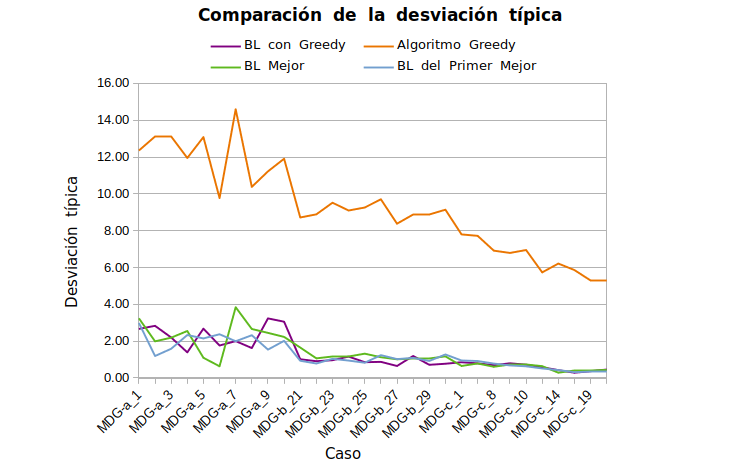
\includegraphics[width=0.9\linewidth]{img/comp_dev}
	\caption{Comparación de la desviación  de los distintos algoritmos para cada caso de estudio}
	\label{fig:compdev}
\end{figure}

\begin{figure}[H]
	\centering
	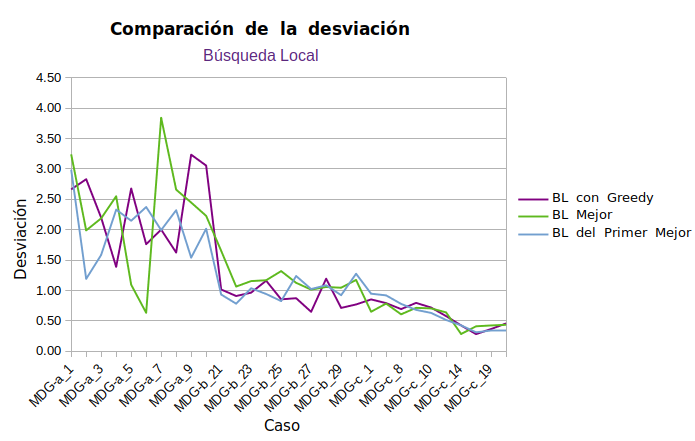
\includegraphics[width=0.9\linewidth]{img/comp_dev_bl}
	\caption{Comparación de la desviación  de los algoritmos de búsqueda local para los distintos casos de estudio}
	\label{fig:compdevbl}
\end{figure}

\begin{figure}[H]
	\centering
	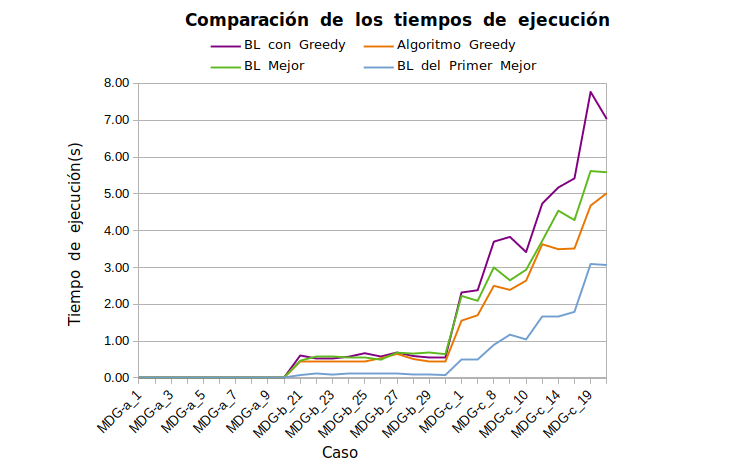
\includegraphics[width=0.9\linewidth]{img/comp_tiempo}
	\caption{Comparación de los tiempos de ejecución de los distintos algoritmos para cada caso de estudio}
	\label{fig:comptiempo}
\end{figure}


	\subsection{ Análisis de los resultados }
	
	Para tener una visión global de los resultados obtenidos por los distintos algoritmos empezamos observando la Tabla 5. Nos damos cuenta de que la búsqueda local del primer mejor presenta la media más baja de la desviación , así como el menor tiempo de ejecución. En el otro extremo tenemos el algoritmo Greedy, que nos da una media de la desviación  muy alta, aunque con un tiempo de ejecución ligeramente menor que las otras dos variantes de la búsqueda local. El algoritmo de la búsqueda local con Greedy es el que tarda más tiempo en ejecutarse en media con diferencia, pero presenta una desviación  casi tan buena como la de la búsqueda local del primer mejor. En un término medio encontramos la búsqueda local del mejor, con una media de la desviación  algo mayor que la obtenida por la BL del primer mejor y un tiempo de ejecución menor que la BL con Greedy pero superior a todos los demás. 
	
	En la Figura 1 apreciamos que el algoritmo Greedy obtiene para todos los casos de estudio una desviación  mucho mayor que los algoritmos de búsqueda local. Esto puede ser debido a que Greedy explora el espacio de soluciones en menor profundidad que los algoritmos de búsqueda local. Además, el criterio elegido en greedy para medir la distancia de un elemento a un conjunto (mínimo de las distancias de ese elemento a los elementos del conjunto) tiene sentido desde el punto de vista matemático, pero para la práctica en este problema no es el criterio más adecuado. Una mejor elección habría sido considerar la suma de las distancias de ese elemento a todos los del conjunto, que es lo que tratamos de maximizar en MDP. 
	
	 Si nos vamos ahora a la Figura 2, donde se comparan las distintas variantes del algoritmo de búsqueda local, vemos que, aunque en media la BL del primer mejor presenta la desviación  más baja, dependiendo del caso es menor la desviación de un algoritmo u otro, sobre todo en los casos de estudio con un tamaño del espacio menor. Este hecho deja claro que la bondad de un algoritmo depende del caso de estudio en el que se aplica. Nos damos cuenta, además, de que la desviación de todos los algoritmos disminuye cuando el tamaño del problema aumenta (valores de $n$ y $m$ más grandes), así como la diferencia entre las desviaciones de los distintos algoritmos. Podemos decir entonces que los algoritmos de BL son más efectivos en problemas grandes. 
	 
	 La búsqueda local del mejor en general encuentra peores soluciones que la búsqueda local del primer mejor, lo cual puede deberse a que el primero pasa a la mejor solución dentro de un entorno sin tener en cuenta el resto del espacio, lo que propicia que el algoritmo se quede atrapado en un máximo local que puede no ser muy bueno ni ser el máximo global. Además, conlleva un mayor tiempo de ejecución, por tener que evaluar en cada iteración todas las posibles soluciones vecinas para buscar la mejor. La única ventaja es que puede encontrar una solución buena en menos iteraciones que la BL del primer mejor, pero al precio de evaluar todas las soluciones vecinas, lo cual hace que esa ventaja no merezca mucho la pena en la mayoría de los casos. En la Figura 3 vemos que efectivamente el tiempo de ejecución de la BL del mejor es en general mayor que el de la BL del primer mejor, principalmente en los problemas más grandes donde el tiempo de ejecución es un aspecto importante a tener en cuenta. 
	 
	 En cuanto al algoritmo de BL del primer mejor partiendo de la solución proporcionada por el algoritmo Greedy, presenta la ventaja de que la solución de partida ya es considerablemente buena, por lo que en pocas iteraciones de la BL del primer mejor se encuentra una solución mejor. Sin embargo, hay que sumar el tiempo de ejecución del propio algoritmo Greedy, que como ya hemos visto es más alto (el doble que el de BL del primer mejor). Si volvemos a fijarnos en la Figura 3, nos damos cuenta de que si 'sumamos las gráficas' de los tiempos de ejecución del algoritmo Greedy y del algoritmo de la BL del primer mejor, el resultado supera a la gráfica del tiempo de ejecución de BL con greedy. No obstante la diferencia es muy pequeña, debido a que las soluciones proporcionadas por Greedy no son demasiado buenas y la BL debe iterar bastantes veces hasta encontrar una solución buena, de manera que una solución aleatoria de partida en este algoritmo tiene casi el mismo efecto que una proporcionada por greedy en cuanto al tiempo de ejecución. 
	 
	 Otra ventaja que puede tener partir de la solución que nos da el algoritmo Greedy es que la BL empieza en una zona del espacio de soluciones donde es más propable que se encuentre la solución óptima, por lo que la BL puede llegar a encontrar una solución mejor que si se partiera de una solución aleatoria, de ahí que para algunos casos de estudio este algoritmo presente una menor desviación (ver Figura 2). Este hecho tendría una mayor influencia si las soluciones que nos da greedy fueran mejores, pues ya hemos visto que en nuestro caso no son muy buenas. 
	 
	 Por lo tanto, la búsqueda local con Greedy en nuestro problema no merece mucho la pena, pues presenta el tiempo de ejecución más alto y no mejora en general las soluciones encontradas partiendo de una solución aleatoria. En problemas en los que se conozca la solución de greedy, de manera que no haya que añadir su tiempo de ejecución al del propio algoritmo, y esta sea considerablemente buena, esta estrategia podría ser efectiva. 
	 
	 Finalmente, vamos a intentar ver por qué el algoritmo Greedy tarda más tiempo en ejecutarse que la búsqueda local del primer mejor. Por una parte, el algoritmo Greedy tiene que recorrer todos los elementos no seleccinados en cada iteración y calcular sus distancias al conjunto de los elementos seleccionados para determinar cuál es el elemento más prometedor para añadir al conjunto. Sin embargo, en la búsqueda local del primer mejor no es necesario recorrer todos los elementos no seleccionados, sino que sólo se recorren hasta encontrar una solución mejor. Por otra parte, en Greedy sólo se calcula la bondad de la solución al final (se llama a la función \lstinline|fitness|), una vez encontrada la misma, mientras que en BL hay que evaluar muchas soluciones intermedias, lo cual es costoso. Sin embargo, la factorización de la función objetivo en BL, hace que estas evaluaciones sean más rápidas pues, como ya vimos, no es necesario calcular el coste de la solución completa, sino solo la contribución del nuevo elemento insertado. 
	 
	 Teniendo en cuenta todos estos aspectos comentados y los resultados propocionados por los algoritmos estudiados, podemos concluir que en este problema el algoritmo de la búsqueda local del primer mejor es más adecuado en general, pues ofrece la menor desviación  en la mayoría de los casos en un tiempo de ejecución muy pequeño. No obstante, hay que tener en cuenta el caso de estudio concreto para decantarse por un algoritmo u otro, pues en algunos casos la búsqueda local del mejor o la BL del primer mejor con greedy encuentran una mejor solución. 
	 

\end{document}